\section{Integers}
\label{sec:orga8b7d2e}

Integers are numbers without a decimal point. There are two types of integers,
signed and unsigned. The type of signed integers starts with the letter
\token{i}, while the type of unsigned integers starts with the letter
\token{u}.

\begin{center}
  \begin{tabular}{|r|ll|}
    \hline
    size & signed & unsigned\\[0pt]
    \hline
    \hline
    8 & \texttt{i8} & \texttt{u8}\\[0pt]
    16 & \texttt{i16} & \texttt{u16}\\[0pt]
    32 & \texttt{i32} & \texttt{u32}\\[0pt]
    64 & \texttt{i64} & \texttt{u64}\\[0pt]
    arch & \texttt{isize} & \texttt{usize}\\[0pt]
    \hline
  \end{tabular}
\end{center}

The size of the type in bits is written in the type itself, e.g. \token{i32} is
a signed int of 32 bits. The table above shows the list of integer types
implemented in version 1.0 of ymirc. \token{usize} and \token{isize} are
architecture dependent and have a size in bits that depends on the size of the
pointers on the target system, (i.e. 32 bits on 32 bit systems, 64 bits on 64
bit systems, and so on).


\vspace{-10pt}%
\subsection{Literals}
\label{sec:org2cf045d}

Integer literals can be written in four forms:
\begin{enumerate}
\item Octal, starting with \token{0o} and containing only numbers between \token{0} and \token{7}. (e.g. \token{0o71217}).
  \vspace{-2pt}%
\item Hexadecimal, starting with \token{0x} and containing numbers from
  \token{0} to \token{9} and letters from \token{a} to \token{f} in upper or
  lower case (e.g. \token{0xAB87fe}).
  \vspace{-2pt}%
\item Binary, starting with \token{0b} and containing numbers from \token{0} to
  \token{1} (e.g. \token{0b10010}).
  \vspace{-2pt}%
\item Decimal, starting with nothing special and containing numbers from
  \token{0} to \token{9} (e.g. \token{182993}).
\end{enumerate}

All four forms can also contain the token \token{\_} to separate long integer
literals and make them more readable (e.g. \token{1\_000\_000\_000\_000}).
There can be as many \token{\_} as you like, they will just be removed during
compilation.

Literals must end with a suffix to define a literal of an int type other than
\token{i32}. For example, to define a literal with value \token{67} and type
\token{i8}, you would write \token{67i8} or \token{0x43i8} or
\token{0o103i8}. A check is made during compilation to ensure that the selected
int type has enough bytes to encode the expected literal. Suffixes for
\token{isize} and \token{usize} are \token{is} and \token{us} respectively.

\subsection{Properties}
\label{sec:orgc02cb40}

Integer properties are accessed using the \token{::} operator (as for any type)
on a type expression. The properties are

\begin{center}
  \vspace{-3pt}
  \begin{adjustbox}{max width=\linewidth}
    \begin{tabular}{|l|ll|}
      \hline
      name & value & type\\[0pt]
      \hline
      \hline
      \texttt{init} & The initial value \texttt{0} & \texttt{typeof(x)}\\[0pt]
      \texttt{max} & The maximum value the type can encode & \texttt{typeof(x)}\\[0pt]
      \texttt{min} & The minimum value the type can encode & \texttt{typeof(x)}\\[0pt]
      \hline
      \texttt{typeid} & A string encoding the name of the type & \texttt{[c8]}\\[0pt]
      \hline
    \end{tabular}
  \end{adjustbox}
\end{center}

\smallskip

The following code shows an example of how type properties can be used.
\smallskip

\begin{lstlisting}[style=coloredverbatim]
  println (i32::max); // 2_147_483_647
  println (i16::min); // -32_768
\end{lstlisting}

\subsection{Casting}
\label{sec:orgfdc3d25}

Integer values can be cast to other types.

\begin{itemize}
\item To other integers: It is impossible to change the type of an int value
implicitly, i.e. it is impossible to transform a value of type \token{i32} into
a value of type \token{i64} without explicitly mentioning it. The cast operator
\token{cast!T (V)} can convert any int type to another int type.


\item To char types: The cast operator can be used to convert an int type of
  type \token{u8} to a \token{c8}, a \token{u32} to a \token{c32} and a
  \token{u16} to a \token{c16} and vice versa (e.g. \token{c8} to
  \token{u8}). This is the only allowed casting from int to chars. Implicit
  casting is not allowed. The transformation does not change the value in any
  way (exactly the same bits before and after the cast).

  \begin{lstlisting}[style=coloredverbatim]
let a : c32 = cast!c32 (97u32);
let b : u8 = cast!u8 ('a'c8);
  \end{lstlisting}

\item To floating-point types: Casting to floating-point types is allowed from
  any int type whose type has a size of at least \token{4} bytes (\token{i32},
  \token{u32} and higher) to any floating-point type, and vice versa using the
  cast operator. This is the only allowed casting from int to float types.
  Implicit casting is not allowed. The value encoding is changed to be
  represented correctly. In fact, int and float have completely different ways
  of representing values in memory. The value is truncated when converted from a
  float to an int. And there may be some stepping when converting an int value
  to a float value, due to the holes in the set of values representable by the
  float encoding system.
  \smallskip

  \begin{lstlisting}[style=coloredverbatim]
let a : f32 = cast!f32 (97u32);
let b : f64 = cast!f64 (12);

let c : i64 = cast!i64 (67.87);
  \end{lstlisting}

\end{itemize}

\subsubsection{Implicit casting}

Implicit casting of integer values is sometimes allowed under certain
conditions. The value must be \token{cte}, and an overflow check is performed
to ensure that it does not overflow the capabilities of the type to which it is
cast.

  \begin{lstlisting}[style=coloredverbatim]
fn foo (a : u64) {
  // ...
}

let a : i64 = 1;
foo (7 + a); // 7 + a can be known at compilation time, 'a' is immutable and cte

let b : usize = 0; // no problem '0' is implicitely converted to 'usize'
  \end{lstlisting}

The purpose of this is to reduce the verbosity of the code when it is not
necessary, and the type is explicitly defined without ambiguity. It is not
possible to implicitly convert values of types other than integers to integer
values (e.g. character literals cannot be implicitly converted to integer
values). Implicit conversion is not allowed in cases of ambiguity. For instance,
in the following source code, there is no definition of the function
\token{foo} that accepts a value of type \token{u8}, so both functions might
work.

\begin{lstlisting}[style=coloredverbatim, escapechar=@]
fn foo (a : i32) {
    println ("foo i32 ", a);
}

fn foo (a : usize) {
    println ("foo usize ", a);
}

fn main () {
    foo (1); // ok, foo i32 1
    foo (1us); // ok, foo usize 1
    @\hb{foo (1u8)}@; // error, works with both
}
  \end{lstlisting}

The compiler rejects the code with an error. If there was only one definition of
the function \token{foo}, the implicit cast would have been allowed (after an
overflow check).

\subsection{Unary operators}
\label{sec:orge691bb5}

The following unary operators can be used on int types.
\smallskip


%% \begin{adjustbox}{max width=\linewidth}
\begin{center}
  \vspace{-5pt}
  \begin{threeparttable}
    \begin{tabular}{|l|ll|}
      \hline
      Operator & Operation & Example\\[0pt]
      \hline
      \hline
      \texttt{-} & Opposite value & \texttt{-19}\\[0pt]
      \hline
      \texttt{!} & Byte Not\(^{1}\) & \texttt{!19 == -20}\\[0pt]
      \hline
    \end{tabular}
    \begin{tablenotes}

    \item[1.] \footnotesize \textit{inverts each bit of the binary
      representation of the int value. This is semantically the same as
      computing \token{-x-1} (if the integer is signed).}

    \end{tablenotes}
  \end{threeparttable}
\end{center}
%% \end{adjustbox}

The result of unary operations always has the same type as the operand used in
the operation. The inverse operator \token{-} cannot be used on unsigned types
because they cannot be negative.

\subsection{Binary operators}
\label{sec:orgb91194f}

Binary operators with an int operand can only be used if both operands are of
type int. There are two exceptions to this rule: 1. When the operation involves
an object operand that has overridden the said binary operator (as a left or
right operand), 2. When one of the operands is of char or pointer type. Binary
operators involving char types are presented in the section on char types
(cf. Section~\ref{sec:char_type}), and those involving pointer types are presented in
the chapter on compound types (cf. Section~\ref{sec:pointer_type}).

The binary operators are divided into 5 groups:

\begin{itemize}
\item Arithmetics: Binary arithmetic operators can be used with two int values
  whose types have the same signed property (two signed operands or two unsigned
  operands, but not a mix). The result of the operation takes the type of the
  largest of the two operands, e.g. for an addition between a \token{i64} and a
  \token{i32} (e.g. \token{12 + 78i64}), the result takes the type
  \token{i64}. There is one exception, the exponent operator, where the right
  operand is always \token{i32} and the result is always of the type of the
  left operand.

  \begin{center}
    \vspace{-10pt}
    \begin{adjustbox}{max width=1.0\linewidth}
      \begin{tabular}{|c|lll|}
        \hline
        Operator & Operation & Commutative & Example\\[0pt]
        \hline
        \hline
        \texttt{+} & Addition & Yes & \texttt{1 + 2 == 3}\\[0pt]
        \texttt{-} & Subtraction & No & \texttt{2 - 1 == 1}\\[0pt]
        \texttt{*} & Multiplication & Yes & \texttt{3 * 4 == 12}\\[0pt]
        \texttt{/} & Division (truncate) & No & \texttt{13 / 3 == 4}\\[0pt]
        \texttt{\%} & Rest of the division & No & \texttt{13 \% 3 == 1}\\[0pt]
        \texttt{\textasciicircum{}\textasciicircum{}} & Exponant & No & \texttt{3\textasciicircum{}\textasciicircum{}4 == 81}\\[0pt]
        \hline
      \end{tabular}
    \end{adjustbox}
  \end{center}

\item Bytes: Bytes binary operators can be used with two int values of exactly
  the same type (e.g. \token{i64} with and only with \token{i64}).

  \begin{center}
    \vspace{-20pt}
    \begin{adjustbox}{max width=1.0\linewidth}
      \begin{tabular}{|c|l l l|}
        \hline
        Operator & Operation & Commutative & Example \\[0pt]
        \hline
        \hline
        \texttt{\(\vert\)} & Byte Or & Yes & \texttt{0b001} \(\vert{}\) \texttt{0b010 == 0b011}\\[0pt]
        \texttt{\&} & Byte And & Yes & \texttt{0b001 \& 0b010 == 0b000}\\[0pt]
        \texttt{\textasciicircum{}} & Byte Xor & Yes & \texttt{0b001 \textasciicircum{} 0b011 == 0b010}\\[0pt]
        \texttt{>>} & Byte left shift & No & \texttt{0b100000 >> 0b010 == 0b001000}\\[0pt]
        \texttt{<<} & Byte right shift & No & \texttt{0b001000 << 0b010 == 0b100000}\\[0pt]
        \hline
      \end{tabular}
    \end{adjustbox}
  \end{center}

\item Logical: Binary logical operators can be used with two integer values
  whose types have the same signed property (two signed operands or two unsigned
  operands, but not a mix). The largest type of the two integers is used to cast
  the value of the operand with the smallest type, to ensure that there is no
  overflow during the comparison. The result of the operation is always of type
  \token{bool}.

  \begin{center}
    \vspace{-20pt}
    \begin{adjustbox}{max width=1.0\linewidth}
      \begin{tabular}{|c|l l l|}
        \hline
        Operator & Operation & Commutative & Example\\[0pt]
        \hline
        \hline
        \texttt{>} & Greater than & No & \texttt{(12 > 11) == true}\\[0pt]
        \texttt{<} & Lower than & No & \texttt{(12 < 11) == false}\\[0pt]
        \texttt{>=} & Greater or equal & No & \texttt{(14 >= 14) == true}\\[0pt]
        \texttt{<=} & Lower or equal & No & \texttt{(11 <= 19) == true}\\[0pt]
        \texttt{==} & Equal & Yes & \texttt{(10 == 10) == true}\\[0pt]
        \texttt{!=} & Not equal & Yes & \texttt{(10 != 10) == false}\\[0pt]
        \hline
      \end{tabular}
    \end{adjustbox}
  \end{center}

\item Affectation: The affectation operator \token{=} can be used when the two
  operands are of exactly the same int type. The left operand must be a mutable
  lvalue (e.g. a mutable variable, a slice access, etc.). The affectation
  operator can be mixed with a math or byte operator (e.g. \token{+=},
  \token{\&=}, etc.). In this case, the operation \token{x += y} is rewritten
  as \token{x = x + (y)}, where the y operand always has a higher priority than
  the affectation operator. For example, the operation \token{x *= 12 + 3} is
  rewritten as \token{x = x * (12 + 3)}, even though the multiplication
  operator has a higher priority than the addition operator, i.e. the result of
  \token{x *= (12 + 3)} is different from the result of \token{x = (x * 12 +
    3)}.

  \begin{lstlisting}[style=coloredverbatim]
let mut a = 11;
let b = a * 12 + 3;
a *= 12 + 3;

assert (b == 135);
assert (a == 165);
  \end{lstlisting}

\item Range: The range operator can be used on int values of exactly the same
  type, creating a \token{range} value. The range type is a native compound
  type, described in the next chapter (cf. Section~\ref{sec:range_type}).

  \begin{center}
    \vspace{-10pt}
    \begin{adjustbox}{max width=1.0\linewidth}
      \begin{tabular}{|c|lll|}
        \hline
        Operator & Operation & Example & Interval\\[0pt]
        \hline
        \texttt{..} & Range operator not inclusive & \texttt{34 .. 12} & \texttt{[34;12[}\\[0pt]
            \texttt{...} & Range operator inclusive & \texttt{5 ... 89} & \texttt{[5;89]}\\[0pt]
            \hline
      \end{tabular}
    \end{adjustbox}
  \end{center}

The value of the result range has a default increment of \token{1} and its
inner type is the type of the operand. It can be ascending or descending
depending on the values used to construct it.

\end{itemize}

\subsection{Overflowing}
\label{sec:org0881da2}

Compile-time checks for value overflow are performed on \textit{cte} values.
There is no way to check for an overflow at runtime, and it may occur.

\begin{figure*}[t]
  \centering
  \scalebox{0.9}{
    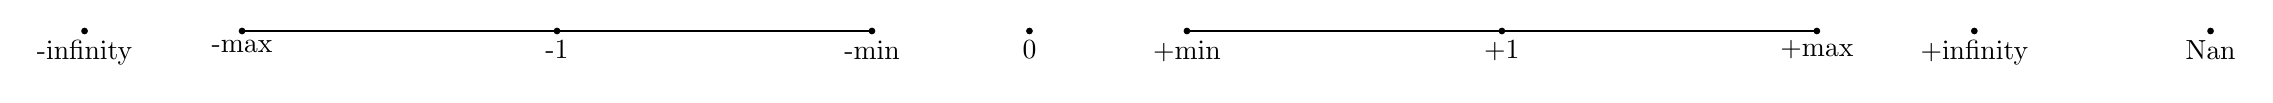
\begin{tikzpicture}
      \filldraw (0,0) circle (1pt) node[align=center, below] {-infinity};
      \filldraw (2,0) circle (1pt) node[align=center, below] {-max};
      \filldraw (6,0) circle (1pt) node[align=center, below] {-1};
      \filldraw (10,0) circle (1pt) node[align=center, below] {-min};
      \filldraw (12,0) circle (1pt) node[align=center, below] {0};
      \filldraw (14,0) circle (1pt) node[align=center, below] {+min};
      \filldraw (18,0) circle (1pt) node[align=center, below] {+1};
      \filldraw (22,0) circle (1pt) node[align=center, below] {+max};
      \filldraw (24,0) circle (1pt) node[align=center, below] {+infinity};
      \filldraw (27,0) circle (1pt) node[align=center, below] {Nan};

      \draw[-](2,0) -- (10, 0);
      \draw[-](14,0) -- (22, 0);

    \end{tikzpicture}
  }
  \caption{\label{float_point_size} Range of representable values with floating point types}
\end{figure*}


\vfill%
\pagebreak

\section{Floating point types}
\label{sec:orgae6ed5f}

Floating point types refer to numbers with a floating decimal point. There are 4
floating point types, shown in the table below. The built-in floating point
types conform to IEEE 754 arithmetic, which means, for example, that
\token{f32} has 1 bit of sign, \token{8} bits of exponent, and \token{24} (23
explicit) bits of mantissa. The \token{fsize} type represents the largest
floating-point type that can be represented on the target architecture.

\begin{center}
  \vspace{-5pt}
  \begin{tabular}{|c|lll|}
    \hline
    type & size & exp & mantissa\\[0pt]
    \hline
    \hline
    \texttt{f32} & 32 & 8 & 24 (23 explicit)\\[0pt]
    \texttt{f64} & 64 & 11 & 53 (52 explicit)\\[0pt]
    \texttt{f80} & 80 & 16 & 64 (63 explicit)\\[0pt]
    \texttt{fsize} & arch & arch & arch\\[0pt]
    \hline
  \end{tabular}
\end{center}

\subsection{Literals}
\label{sec:orgfd9f825}

Floating point types can be written in three different forms, decimal,
scientific notation.

\begin{enumerate}
\item Decimal, two decimal int literals separated by the token \token{.} (with
  no spaces in between). \token{1837.0289}. The decimal part can be omitted,
  which means it is equal to \token{0} (e.g. \token{10.} is valid, but not
  \token{.10}).

\item Scientific notation, similar to decimal notation, but ending with an
  exponent preceded by the letter \token{e} or \token{E}. \token{3.14e78 ==
    (3.14 * 10.0 \textasciicircum{}\textasciicircum{} 78)}, which is \(3.14
  \times 10^{78}\). A sign for the exponential part can be set after the letter
  \token{e} or \token{E} with the token \token{-} or \token{+}, e.g.
  \token{3.e-10}. There must be no spaces in the literal.

\item Hexadecimal notation, starting with \token{0x}, then two hexadecimal int
  literal separated by the \token{.} token, followed by the letter \token{p}
  or \token{P}, and ending with a decimal int literal representing the
  exponential part. The fractional part can be empty, in which case the letter
  \token{p} follows the \token{.} token. However, the \token{.} token and the
  \token{p} exponential part are mandatory. A sign for the exponential part can
  be set after the letter \token{p} or \token{P} with the token \token{-} or
  \token{+}. There can be no spaces in the literal. Unlike scientific notation,
  the exponential part is a power of \token{2} instead of \token{10}, e.g.
  \token{0xA.p4 == (10.0 * 2.0\textasciicircum{}\textasciicircum{}4)}.

\end{enumerate}

The three forms can also contain the token \token{\_} to split long literals
and make them easier to read (e.g. \token{124\_732.789\_281},
\token{0x1.FFFF\_FFFFp1023}, \token{3.14\_15\_92e3f}). There can be as many
\token{\_} as you like, they will just be removed during compilation. Literals
can end with a suffix to specify the type of the literal; \token{f} to define
\token{f32} literals, \token{d} to define \token{f64} (for \token{double}),
\token{l} for \token{f80} (for \token{long}) and \token{r} for
\token{fsize} (for \token{real}). Literals without a suffix are considered to
be of type \token{f64}. The literals \token{4.5e10f} and \token{0.8f},
\token{0x1.FFp10f} are of type \token{f32} and \token{4.5e10} and
\token{0.8}, \token{0x1.FFp10} are of type \token{f64}.

\subsection{Properties}
\label{sec:org52a5d6e}

Floating point properties can be accessed by using the \token{::} operator on a
type expression. The properties are as follows:

\begin{center}
  \vspace{-5pt}
  \begin{adjustbox}{max width=1.01\linewidth}
    \begin{threeparttable}
      \begin{tabular}{|l|ll|}
        \hline
        Name & Meaning & Type\\[0pt]
        \hline
        \hline
        \texttt{init} & The initial value - nan (Not a Number) & \texttt{typeof(x)}\\[0pt]
        \Xhline{0.001pt}
        \texttt{max} & The maximal finite value & \texttt{typeof(x)}\\
        & that this type can encode & \\[0pt]
        \Xhline{0.001pt}

        \texttt{min} & The minimal finite value & \texttt{typeof(x)}\\
        & that this type can encode & \\[0pt]
        \Xhline{0.001pt}

        \texttt{nan} & The value Not a Number & \texttt{typeof(x)}\\[0pt]
        \Xhline{0.001pt}
        \texttt{inf} & The value positive infinity & \texttt{typeof(x)}\\[0pt]
        \Xhline{0.001pt}
        \texttt{epsilon} & The smallest increment & \texttt{typeof(x)}\\
        & to the value 1 &\\[0pt]
        \Xhline{0.001pt}
        \texttt{dig} & The number of decimal digit of precision & \texttt{u32}\\[0pt]
        \Xhline{0.001pt}
        \texttt{mant\_dig} & Number of bits in the mantissa & \texttt{u32}\\[0pt]
        \Xhline{0.001pt}
        \texttt{max\_10\_exp} & The maximum value &  \texttt{i32} \\
        & such that \(10^{max\_10\_exp}\) is representable &\\[0pt]
        \Xhline{0.001pt}
        \texttt{max\_exp} & The maximum value & \texttt{i32}\\
        & such that \(2^{max\_exp-1}\) is representable & \\[0pt]
        \Xhline{0.001pt}
        \texttt{min\_10\_exp} & The minimum value & \texttt{i32}\\
        & such that \(10^{min\_10\_exp}\) is representable$^1$  & \\[0pt]
        \Xhline{0.001pt}
        \texttt{min\_exp} & The minimum value & \texttt{i32}\\
        & such that \(2^{min\_exp-1}\) is representable$^1$ & \\[0pt]
        \hline
        \texttt{typeid} & A string encoding the name of the type & \texttt{[c8]}\\[0pt]
        \hline
      \end{tabular}
      \begin{tablenotes}
      \item[1.] \small \textit{as a normalized value}
      \end{tablenotes}
    \end{threeparttable}
  \end{adjustbox}
\end{center}

\smallskip

\cautionbox { The \texttt{min} value is not the opposite of the \texttt{max}
  value. Figure~\ref{float_point_size} describes the ordering relationship
  between values of floating-point types, where points and lines are the values
  that can be represented by a floating-point type. }

\subsection{Casting}
\label{sec:org9eacb07}

Floating point values can be cast to other types.

\begin{itemize}
\item To other floating-point types: It is impossible to change the type of a
  float implicitly. The cast operator \token{cast!T (V)} can convert any float
  value to another float value of another float type. Because float values of
  different float types are coded with different numbers of bits, there may be
  stepping during casting.

\item To integer types: The cast operator can be used to convert a float value
  of any float type to an int value whose type is at least 4 bytes in size
  (\token{i32}, \token{u32} and larger). If the cast operator is used, the
  value is truncated to the floor value (e.g. \token{1.3} \token{1.5} and
  \token{1.8} are all truncated to \token{1}), and anything that was part of
  the decimal part of the float is lost. The reverse cast is also allowed (from
  any int type whose size is at least \token{4} bytes to any float type); in
  this case, some stepping may occur due to the floating-point encoding.

\end{itemize}

Floating point values cannot be converted to other types.
\subsubsection{Implicit casting}

The implicit casting of float values known at \token{cte} follows the same
rules as described for integer \token{cte} values.

\begin{lstlisting}[style=coloredverbatim, escapechar=@]
fn foo (f : f32) {}
fn foo (f : f64) {}

let a : f32 = 1.0; // ok, f64 is converted implicitely to f32

foo (1.0); // ok, using f64 definition
@\hb{foo (1.0r)}@; // error, both definitions work
\end{lstlisting}

\subsection{Unary operators}
\label{sec:org30770bf}

The \token{-} unary operators can be used on floating point types. The result
of the operation is the opposite value and is of the same type as the operand of
the operation. For example, \token{-89.0f} is of type \token{f32}.

\subsection{Binary operators}
\label{sec:orga43d13a}

Binary operators involving a float operand can only be used if both operands are
floats. There is an exception to this rule when the operation involves an object
operand that has overridden the said binary operator (as a left or right
operand). The binary operators are divided into 4 groups:

\begin{itemize}
\item Arithmetic: Binary arithmetic operators can be used with two float values.
  The result of the operation takes the type of the largest operand (e.g. an
  operation with \token{f32} and \token{f64} takes the type \token{f64}). The
  operators that can be used are described in the table below.

  \begin{center}
    \vspace{-20pt}
    \begin{adjustbox}{max width=1.0\linewidth}
      \begin{tabular}{|c|lll|}
        \hline
        Operator & Operation & Commutative & Example\\[0pt]
        \hline
        \hline
        \texttt{+} & Addition & Yes & \texttt{1.0 + 2.3 == 3.3}\\[0pt]
        \texttt{-} & Subtraction & No & \texttt{1. - 8. == -7.}\\[0pt]
        \texttt{*} & Multiplication & Yes & \texttt{3. * 4. == 12.}\\[0pt]
        \texttt{/} & Division & No & \texttt{7. / 3. == 2.333}\\[0pt]
        \texttt{\%} & Rest of division & No & \texttt{7.23 \% 3.09 == 1.05}\\[0pt]
        \texttt{\textasciicircum{}\textasciicircum{}} & Exponant & No & \texttt{7. \textasciicircum{}\textasciicircum{} 3 == 343.}\\[0pt]
        \hline
      \end{tabular}
    \end{adjustbox}
  \end{center}

  The power operator \token{\textasciicircum{}\textasciicircum{}} is a special
  operator that can take a float or an integer as its right operand. If both
  operands are floats, then they must be of exactly the same type, and the
  result value takes the type of the operands. If the right operand is an int
  value, then the result of the operation takes the type of the left operand.

\item Logical: Binary logical operators can be used with two float values. The
  largest type of the two operands is used to cast the value of the operand with
  the smallest type, to avoid too much stepping (although stepping may still
  occur). The result of the operation is always of type \token{bool}.

  \begin{center}
    \vspace{-20pt}
    \begin{adjustbox}{max width=1.0\linewidth}
      \begin{tabular}{|c|lll|}
        \hline
        Operator & Operation & Commutative & Example\\[0pt]
        \hline
        \hline
        \texttt{>} & Greater than & No & \texttt{(12. > 11.) == true}\\[0pt]
        \texttt{<} & Lower than & No & \texttt{(12. < 11.) == false}\\[0pt]
        \texttt{>=} & Greater or equal & No & \texttt{(14. >= 14.) == true}\\[0pt]
        \texttt{<=} & Lower or equal & No & \texttt{(11. <= 19.) == true}\\[0pt]
        \texttt{==} & Equal & Yes & \texttt{(10. == 10.) == true}\\[0pt]
        \texttt{!=} & Not equal & Yes & \texttt{(10. != 10.) == false}\\[0pt]
        \texttt{<=>} & Is congruent & Yes & \texttt{(10. <=> 10.) == true}\\[0pt]
        \texttt{<!>} & Is not congruent & Yes & \texttt{(10. <!> 10.) == false}\\[0pt]
        \hline
      \end{tabular}
    \end{adjustbox}
  \end{center}

   \token{<=>} and \token{<!>} are special floating point operators designed
   to evaluate the equality and inequality of left and right operands, taking
   into account the possibility of stepping. In other words, it uses the
   \token{::epsilon} value of the floating point type (of the largest operand)
   to evaluate whether the left operand is equal to the right operand delta the
   epsilon value. They also check for \token{nan} equality and inequality.
   These operators are of course less efficient than the equality and inequality
   operators, as they involve multiple instructions and possibly conditional
   jumps.

\item Affectation: The affectation operator \token{=} can be used when the two
  operands are of exactly the same float type. The left operand must be a
  mutable lvalue (e.g. a mutable variable, a slice access, etc.). The
  affectation operator can be mixed with an arithmetic operator (e.g.
  \token{+=}, \token{/=}, etc.). In this case, the operation \token{x += y}
  is rewritten as \token{x = x + (y)}, where the y operand always has a higher
  priority than the affectation operator. For example, the operation \token{x
    *= 12. + 3.} is rewritten as \token{x = x * (12. + 3.)}, even though the
  multiplication operator has a higher priority than the addition operator, i.e.
  the result of \token{x *= (12. + 3.)} is different from the result of
  \token{x = (x * 12. + 3.)}.

  \begin{lstlisting}[style=coloredverbatim]
let mut a = 11.0;
let b = a * 12.0 + 3.0;
a *= 12.0 + 3.0;

assert (b == 135.0);
assert (a == 165.0);
  \end{lstlisting}

\item Range: The range operator can be used on two float values of exactly the
  same type, creating a \token{range} value. The range type is a native
  compound type, which is described in the following chapter (see
  section~\ref{sec:range_type}).

  \begin{center}
    \vspace{-20pt}
    \begin{adjustbox}{max width=1.0\linewidth}
      \begin{tabular}{|l|lll|}
        \hline
        Operator & Operation & Example & Interval\\[0pt]
        \hline
        \hline
        \texttt{..} & Range operator not inclusive & \texttt{34.f .. 12.f} & \texttt{[34.f;12.f[}\\[0pt]
            \texttt{...} & Range operator inclusive & \texttt{5.f ... 89.f} & \texttt{[5.f;89.f]}\\[0pt]
            \hline
      \end{tabular}
    \end{adjustbox}
  \end{center}


  The value of the result range has a default increment of \token{1.0} and its
  inner type is the type of the operand. It can be ascending or descending
  depending on the values used to construct it.

\end{itemize}

\subsection{Overflowing and stepping}
\label{sec:orgd5d9f51}

Because of the way float values are encoded, there are gaps in the set of values
they can represent. Thus, some operations that should be mathematically
equivalent do not always produce the same float value. To compare two float
values, the property \token{::epsilon} can be used, as well as the congruent
operators \token{<=>} and \token{<!>}. There is no value overflow checking
at compile time or runtime.

\vfill%
\pagebreak

\section{Characters}
\label{sec:char_type}

Character types are used to encode characters (ASCII or Unicode). There are
three character types \token{c8}, \token{c16} and \token{c32} with a size of
\token{8}, \token{16} and \token{32} bits respectively. These char types are
encoding values in utf-8, utf-16 and utf-32.

\begin{center}
  \vspace{-5pt}
  \begin{tabular}{ll}
    Value & Content\\[0pt]
    \hline
    \texttt{\textbackslash{}a} & Alert beep, (Bell)\\[0pt]
    \texttt{\textbackslash{}b} & Backspace\\[0pt]
    \texttt{\textbackslash{}f} & Page break\\[0pt]
    \texttt{\textbackslash{}n} & New line\\[0pt]
    \texttt{\textbackslash{}r} & Carriage return\\[0pt]
    \texttt{\textbackslash{}t} & Horizontal tab\\[0pt]
    \texttt{\textbackslash{}v} & Vertical tab\\[0pt]
    \texttt{\textbackslash{}\textbackslash{}} & Backslash\\[0pt]
    \texttt{\textbackslash{}'} & Apostrophe\\[0pt]
    \texttt{\textbackslash{}"} & Double quotation mark\\[0pt]
    \texttt{\textbackslash{}u\{\}} & Unicode\\[0pt]
  \end{tabular}
  \captionof{table}{\label{tab:escape_chars} Escape characters}
\end{center}

\subsection{Properties}
\label{sec:orgf9fbc31}

The properties of char types can be accessed by using the \token{::} operator
on a type expression. The properties are as follows:

\begin{center}
  \vspace{-5pt}
  \begin{adjustbox}{max width=\linewidth}
    \begin{tabular}{|l|ll|}
      \hline
      Name & Meaning & Type\\[0pt]
      \hline
      \hline
      \texttt{init} & The initial value \texttt{\textbackslash{}u\{0\}} & \texttt{typeof(x)}\\[0pt]
      \hline
      \texttt{typeid} & A string encoding the name of the type & \texttt{[c8]}\\[0pt]
      \hline
    \end{tabular}
  \end{adjustbox}
\end{center}


\subsection{Literals}
\label{sec:org73c4919}

Char literals are enclosed by the token \token{'} and can be described using three forms:

\begin{enumerate}
\item Using the direct representation of the character (e.g. \token{π}),
\item Using an escape character. The escape chars are described in the
  table~\ref{tab:escape_chars}.

\item Using an int literal representation of Unicode. To avoid confusing the int
  literal representation with the literal of the int itself, the int literal
  must be encoded using the escape character \token{\textbackslash{}u} and the
  tokens \token{\{} and \token{\}}. For example
  \token{\textbackslash{}u\{0x263A\}}, \token{\textbackslash{}u\{0b1101\}} or
  \token{\textbackslash{}u\{10\}}.

\end{enumerate}

As with float or int literals, a suffix must be added at the end of the literal
to define the value with the correct type. For example, to define a \token{c32}
value containing the character \token{a}, write \token{'a'c32}. Literal values
without a suffix are considered to be of type \token{c8}.

\begin{lstlisting}[style=coloredverbatim]
let a : c32 = 'r'c32;
let b : c8 = '\u{10}';
let d = 'π'c32;
let e = '\n'c8;

assert (e == b);
\end{lstlisting}

\subsection{Casting}
\label{sec:org16d703f}

Char types can be cast using the cast operator. It is not possible to implicitly convert a char value to a value of another type.

\begin{itemize}
\item To other char types: The cast operator can be used to convert a char of
  one size to a char of another size. This does not guarantee encoding validity.
  The standard library defines more complex transformations that respect
  encoding in the \token{std::conv} module.

\item To integer types: The cast operator can be used to transform a char value
  of type \token{c8} into a \token{u8}, a \token{c16} into a \token{u16} and
  a \token{c32} into a \token{u32}. The transformation does not change the
  value in any way (exactly the same bits before and after the cast).

\end{itemize}


\subsubsection{Implicit casting}

The implicit casting of char values known at \token{cte} follows the same
rules as described for integer \token{cte} values.

\begin{lstlisting}[style=coloredverbatim, escapechar=@]
fn foo (f : c32) {}
fn foo (f : c8) {}

let a : c8 = 'a'c32; // ok, c32 is converted implicitely to c8

foo ('a'); // ok, using c8 definition
@\hb{foo ('a'c16)}@; // error, both definitions work
\end{lstlisting}

\subsection{Unary operators}
\label{sec:org78546fb}

No unary operators can be used on char types.

\subsection{Binary operators}
\label{sec:orge863f7d}

Binary operators on character types are divided into four groups.

\begin{itemize}
\item Arithmetic: Binary arithmetic operators can be used with a char value and
  an unsigned int value (of the same size, e.g. for \token{c8} and
  \token{u8}). The result always takes the type of the char operand. It is
  impossible to add or subtract two char values, even if they are of exactly the
  same type.

  \begin{center}
    \vspace{-5pt}\begin{adjustbox}{max width=1.0\linewidth}
      \begin{tabular}{|c|lll|}
        \hline
        Operator & Operation & Commutative & Example\\[0pt]
        \hline
        \hline
        \texttt{+} & Addition & Yes & \texttt{'a' + 16u8 == 'q'}\\[0pt]
        \texttt{-} & Subtraction & No & \texttt{'q' - 16u8 == 'a'}\\[0pt]
        \hline
      \end{tabular}
  \end{adjustbox}\end{center}


  Char values can be used as right operands in arithmetic operations. The type of
  the result operation would still be the type of the char operand, and the int
  operand would still have to be of the same size as the char operand, so
  \token{('q' + 12u8) == (12u8 + 'q')}.

\item Logical: Binary logical operators can be used with two char values of
  exactly the same type. The result of the operation is always of type
  \token{bool}.

  \begin{center}
    \vspace{-10pt}\begin{adjustbox}{max width=1.0\linewidth}
      \begin{tabular}{|c|lll|}
        \hline
        Operator & Operation & Commutative & Example\\[0pt]
        \hline
        \hline
        \texttt{>} & Greater than & No & \texttt{('q' > 'a') == true}\\[0pt]
        \texttt{<} & Lower than & No & \texttt{('q' < 'a') == false}\\[0pt]
        \texttt{>=} & Greater or equal & No & \texttt{('q' >= 'q') == true}\\[0pt]
        \texttt{<=} & Lower or equal & No & \texttt{('b' <= 'r') == true}\\[0pt]
        \texttt{==} & Equal & Yes & \texttt{('a' == 'a') == true}\\[0pt]
        \texttt{!=} & Not equal & Yes & \texttt{('a' != 'a') == false}\\[0pt]
        \hline
      \end{tabular}
  \end{adjustbox}\end{center}

\item Affectation: The affectation operator \token{=} is usable when the left
  operand is a mutable lvalue and the right operand is strictly the same char
  type as the left operand.

  The affectation operator can be mixed with an arithmetic operator \token{+=}
  and \token{-=}, in which case the right operand must be a value whose type is
  an unsigned int with a size exactly equal to the size of the char type of the
  left operand. The affectation \token{x += y} is rewritten as \token{x = x +
    (y)}, where the y operand always has a higher priority than the affectation
  operator.

  \begin{lstlisting}[style=coloredverbatim]
let mut a = 'a';

let b = a + 21u8;

a = 'e';
a += 7u8;

assert (b == 'v');
assert (a == 'l')
  \end{lstlisting}

\item Range: The range operator can be used on two char values whose types are
  strictly identical, creating a range value.

  \begin{center}
    \vspace{-10pt}\begin{adjustbox}{max width=1.0\linewidth}
      \begin{tabular}{|l|lll|}
        \hline
        Operator & Operation & Example & Interval\\[0pt]
        \hline
        \hline
        \texttt{..} & Range operator not inclusive & \texttt{'a' .. 'z'} & \texttt{[a;z[}\\[0pt]
            \texttt{...} & Range operator inclusive & \texttt{'a' ... 'r'} & \texttt{[a;r]}\\[0pt]
            \hline
      \end{tabular}
  \end{adjustbox}\end{center}


  The result value has a default increment of \token{1} and its inner type is
  the type of the operands. It can be increasing or decreasing depending on the
  values used to construct it.

\end{itemize}

\subsection{Overflowing}
\label{sec:orga9c18c5}

Compile time overflow checking is done on \textit{cte} values. The check ensures
that the chosen type is large enough to encode the value. There is no way to
check for overflow at runtime, and it can happen. It is also possible, due to
the encoding, that a value is not a valid unicode or ascii value if it is
created at runtime (e.g. \token{'π' + 501u32}).

\vfill%
\pagebreak

\section{Boolean}
\label{sec:org9f3a743}

The Bool type is a simple type, whose name is \token{bool}, and that can only
describe two values \token{true} and \token{false}. It is stored in a single
byte of memory, although only the first bit is used and has meaning.

\subsection{Properties}
\label{sec:org503bc9e}

Properties of the type \token{bool} are accessible by using the operator
\token{::} on a type expression. The properties are as follows:

\begin{center}
  \vspace{-5pt}
  \begin{adjustbox}{max width=\linewidth}
    \begin{tabular}{|l|ll|}
      \hline
      Name & Meaning & Type\\[0pt]
      \hline
      \hline
      \texttt{init} & The initial value \texttt{false} & \texttt{bool}\\[0pt]
      \hline
      \texttt{typeid} & A string encoding the name of the type & \texttt{[c8]}\\[0pt]
      \hline
    \end{tabular}
  \end{adjustbox}
\end{center}

\subsection{Literals}
\label{sec:org7620b9c}

Boolean literals are the keywords \token{true} and \token{false}.

\subsection{Casting}
\label{sec:org7cd1f94}

A value of type \token{bool} can be cast to a value of type \token{u8} using
the cast operator, in which case the value \token{false} is converted to the
value \token{0u8} and the value \token{true} is converted to the value
\token{1u8}. The reverse conversion is impossible using the cast operator, but
can be carried out using the equality operators of type int (e.g. \token{1u8 ==
  1u8}). This is the only cast allowed for the boolean type. It is impossible to
convert a boolean value to a value of another type without explicitly using the
cast operator.

\subsection{Unary operators}
\label{sec:orgb412ce4}

The unary operator \token{!} can be used on a boolean value to get its opposite
value (i.e. \token{!true} becomes \token{false} and \token{!false} becomes
\token{true}).

\subsection{Binary operators}
\label{sec:org030ae50}

Binary operators involving a bool operand can only be used if both operands are
of type bool. There is an exception to this rule when the operation involves an
object operand that has overridden the said operator (as a left or right
operand).

Binary operators are divided into 3 groups:

\begin{itemize}
\item Affectation: Affectation operators can be used to change the value of a
  mutable lvalue of type bool using a right operand of type bool. Because there
  are no arithmetic operators that can be used on a bool value, no arithmetic
  operator can be attached to the affectation operation. \token{\&\&=} and
  \token{||=} are not valid operators, and their use results in a syntax error.

\item Comparisons: The comparison operators \token{==} and \token{!=} can be
  used with two bool values to evaluate equality and inequality respectively.
  The result of the operations is always of type \token{bool}. By convention,
  it is not recommended to use equality and inequality operators to test the
  \token{bool} values. In fact, \token{a == false} can be rewritten as
  \token{!a}, and \token{a == true} is simply \token{a}.

\item Logical: Logical operators can be used with two bool operands.

  \begin{center}
    \vspace{-20pt}
    \begin{adjustbox}{max width=1.0\linewidth}
      \begin{tabular}{|c|l l l|}
        \hline
        Operator & Operation & Commutative & Example\\[0pt]
        \hline
        \hline
        \texttt{\(\vert\vert\)} & Or & No & \texttt{false} \(\vert{} \vert{}\) \texttt{true == true}\\[0pt]
        \texttt{\&\&} & And & No & \texttt{true \&\& false == false}\\[0pt]
        \hline
      \end{tabular}
    \end{adjustbox}
  \end{center}

  The operators \token{\&\&} and \token{||} are marked as non-commutative. This
  is not because they can return a different value if the left and right operands
  are inverted, but because for \token{\&\&} the right operand is not evaluated
  if the left operand is false, and for \token{||} the right operand is not
  evaluated if the left operand is true. This can be useful when chaining tests.

  \begin{lstlisting}[style=coloredverbatim]
let i = 12;
let p = &i;

// if 'p == null', '*p == 12' is not evaluated
let a = p != null && *p == 12;

// if 'p == null', '*p != 12' is not evaluated
let b = p == null || *p != 12;

// foo function is not called
let c = true || foo ();

// foo function is called
let d = false || foo ();
  \end{lstlisting}
\end{itemize}

\section{Void}
\label{sec:org409c2d8}

The \token{void} type is a special type that has no value and occupies
\token{0} byte of memory. Unlike other types, it cannot be used to declare
variables. There is no literal to describe a void type, as it cannot take a
value. There is no way to cast a void type to another type, there is no value to
transform. For the same reason, there are no operators applicable to void types.

\vspace{-10pt}
\subsection{Properties}
\label{sec:orgffa98ee}

The properties of a void type can be accessed by using the \token{::} operator
on a type expression. The properties are:

\begin{center}
  \vspace{-5pt}
  \begin{adjustbox}{max width=\linewidth}
    \begin{tabular}{|l|ll|}
      \hline
      Name & Meaning & Type\\[0pt]
      \hline
      \hline
      \texttt{typeid} & A string encoding the name of the type & \texttt{[c8]}\\[0pt]
      \hline
    \end{tabular}
  \end{adjustbox}
\end{center}
